%% This file was auto-generated by IPython.
%% Conversion from the original notebook file:
%% meanshift.ipynb
%%
\documentclass[11pt,english,fleqn]{article}

%% This is the automatic preamble used by IPython.  Note that it does *not*
%% include a documentclass declaration, that is added at runtime to the overall
%% document.

\usepackage{amsmath}
\usepackage{amssymb}
\usepackage{graphicx}
\usepackage{ucs}
\usepackage[utf8x]{inputenc}

% needed for markdown enumerations to work
\usepackage{enumerate}

% Slightly bigger margins than the latex defaults
\usepackage{geometry}
\geometry{verbose,tmargin=3cm,bmargin=3cm,lmargin=2.5cm,rmargin=2.5cm}

% Define a few colors for use in code, links and cell shading
\usepackage{color}
\definecolor{orange}{cmyk}{0,0.4,0.8,0.2}
\definecolor{darkorange}{rgb}{.71,0.21,0.01}
\definecolor{darkgreen}{rgb}{.12,.54,.11}
\definecolor{myteal}{rgb}{.26, .44, .56}
\definecolor{gray}{gray}{0.45}
\definecolor{lightgray}{gray}{.95}
\definecolor{mediumgray}{gray}{.8}
\definecolor{inputbackground}{rgb}{.95, .95, .85}
\definecolor{outputbackground}{rgb}{.95, .95, .95}
\definecolor{traceback}{rgb}{1, .95, .95}

% Framed environments for code cells (inputs, outputs, errors, ...).  The
% various uses of \unskip (or not) at the end were fine-tuned by hand, so don't
% randomly change them unless you're sure of the effect it will have.
\usepackage{framed}

% remove extraneous vertical space in boxes
\setlength\fboxsep{0pt}

% codecell is the whole input+output set of blocks that a Code cell can
% generate.

% TODO: unfortunately, it seems that using a framed codecell environment breaks
% the ability of the frames inside of it to be broken across pages.  This
% causes at least the problem of having lots of empty space at the bottom of
% pages as new frames are moved to the next page, and if a single frame is too
% long to fit on a page, will completely stop latex from compiling the
% document.  So unless we figure out a solution to this, we'll have to instead
% leave the codecell env. as empty.  I'm keeping the original codecell
% definition here (a thin vertical bar) for reference, in case we find a
% solution to the page break issue.

%% \newenvironment{codecell}{%
%%     \def\FrameCommand{\color{mediumgray} \vrule width 1pt \hspace{5pt}}%
%%    \MakeFramed{\vspace{-0.5em}}}
%%  {\unskip\endMakeFramed}

% For now, make this a no-op...
\newenvironment{codecell}{}

 \newenvironment{codeinput}{%
   \def\FrameCommand{\colorbox{inputbackground}}%
   \MakeFramed{\advance\hsize-\width \FrameRestore}}
 {\unskip\endMakeFramed}

\newenvironment{codeoutput}{%
   \def\FrameCommand{\colorbox{outputbackground}}%
   \vspace{-1.4em}
   \MakeFramed{\advance\hsize-\width \FrameRestore}}
 {\unskip\medskip\endMakeFramed}

\newenvironment{traceback}{%
   \def\FrameCommand{\colorbox{traceback}}%
   \MakeFramed{\advance\hsize-\width \FrameRestore}}
 {\endMakeFramed}

% Use and configure listings package for nicely formatted code
\usepackage{listingsutf8}
\lstset{
  language=python,
  inputencoding=utf8x,
  extendedchars=\true,
  aboveskip=\smallskipamount,
  belowskip=\smallskipamount,
  xleftmargin=2mm,
  breaklines=true,
  basicstyle=\small \ttfamily,
  showstringspaces=false,
  keywordstyle=\color{blue}\bfseries,
  commentstyle=\color{myteal},
  stringstyle=\color{darkgreen},
  identifierstyle=\color{darkorange},
  columns=fullflexible,  % tighter character kerning, like verb
}

% The hyperref package gives us a pdf with properly built
% internal navigation ('pdf bookmarks' for the table of contents,
% internal cross-reference links, web links for URLs, etc.)
\usepackage{hyperref}
\hypersetup{
  breaklinks=true,  % so long urls are correctly broken across lines
  colorlinks=true,
  urlcolor=blue,
  linkcolor=darkorange,
  citecolor=darkgreen,
  }

% hardcode size of all verbatim environments to be a bit smaller
\makeatletter 
\g@addto@macro\@verbatim\small\topsep=0.5em\partopsep=0pt
\makeatother 

% Prevent overflowing lines due to urls and other hard-to-break entities.
\sloppy

\setlength{\mathindent}{0pt}
\setlength{\parindent}{0pt}
\setlength{\parskip}{8pt}
\begin{document}

Ortalama Kaydirma ile Kumeleme (Mean Shift Clustering)

Kumeleme yapmak icin bir metot daha: Ortalama Kaydirma metotu. Bu
metodun mesela K-Means'den farki kume sayisinin onceden belirtilmeye
ihtiyaci ol\textbf{ma}masidir, kume sayisi otomatik olarak metot
tarafindan saptanir.

``Kume'' olarak saptanan aslinda veri icindeki tum yogunluk bolgelerinin
merkezleridir, yani alttaki resmin sag kismindaki bolgeler.

\begin{codecell}
\begin{codeinput}
\begin{lstlisting}
im=imread("dist.png"); imshow(im)
\end{lstlisting}
\end{codeinput}
\begin{codeoutput}
\begin{verbatim}
<matplotlib.image.AxesImage at 0xa3f3c4c>
\end{verbatim}
\begin{center}
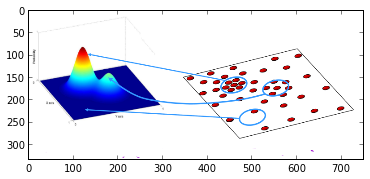
\includegraphics[width=0.7\textwidth]{meanshift_files/meanshift_fig_00.png}
\par
\end{center}
\end{codeoutput}
\end{codecell}
Baslangic neresidir? Baslangic tum noktalardir, yani her noktadan
baslanarak

\begin{enumerate}[1.]
\item
  O nokta etrafinda (yeterince buyuk) bir pencere tanimla
\item
  Bu pencere icine dusen tum noktalari hesaba katarak bir ortalama yer
  hesapla
\item
  Pencereyi yeni ortalama noktayi merkezine alacak sekilde kaydir
\end{enumerate}
Metotun ismi buradan geliyor, cunku pencere yeni ortalamaya dogru
``kaydiriliyor''. Altta bir noktadan baslanarak yapilan hareketi
goruyoruz. Kaymanin saga dogru olmasi mantikli cunku tek pencere icinden
bakinca bile yogunlugun ``sag tarafa dogru'' oldugu gorulmekte. Yontemin
puf noktasi burada.

\begin{codecell}
\begin{codeinput}
\begin{lstlisting}
im=imread("mean_2.png"); imshow(im)

\end{lstlisting}
\end{codeinput}
\begin{codeoutput}
\begin{verbatim}
<matplotlib.image.AxesImage at 0x9b966ac>
\end{verbatim}
\begin{center}
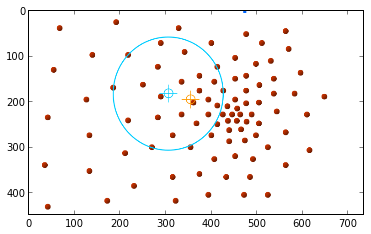
\includegraphics[width=0.7\textwidth]{meanshift_files/meanshift_fig_01.png}
\par
\end{center}
\end{codeoutput}
\end{codecell}
\begin{codecell}
\begin{codeinput}
\begin{lstlisting}
im=imread("mean_3.png"); imshow(im)

\end{lstlisting}
\end{codeinput}
\begin{codeoutput}
\begin{verbatim}
<matplotlib.image.AxesImage at 0x9cd99ec>
\end{verbatim}
\begin{center}
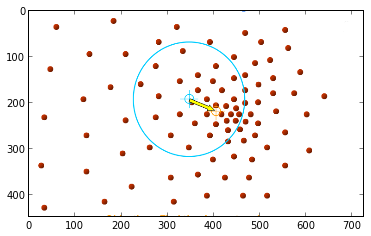
\includegraphics[width=0.7\textwidth]{meanshift_files/meanshift_fig_02.png}
\par
\end{center}
\end{codeoutput}
\end{codecell}
\begin{codecell}
\begin{codeinput}
\begin{lstlisting}
im=imread("mean_4.png"); imshow(im)

\end{lstlisting}
\end{codeinput}
\begin{codeoutput}
\begin{verbatim}
<matplotlib.image.AxesImage at 0x9e3cfac>
\end{verbatim}
\begin{center}
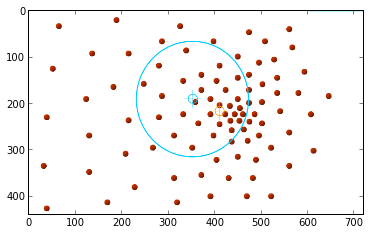
\includegraphics[width=0.7\textwidth]{meanshift_files/meanshift_fig_03.png}
\par
\end{center}
\end{codeoutput}
\end{codecell}
\begin{codecell}
\begin{codeinput}
\begin{lstlisting}
im=imread("mean_5.png"); imshow(im)

\end{lstlisting}
\end{codeinput}
\begin{codeoutput}
\begin{verbatim}
<matplotlib.image.AxesImage at 0x9f9b5ec>
\end{verbatim}
\begin{center}
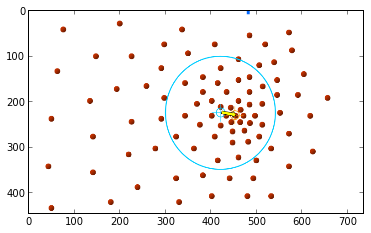
\includegraphics[width=0.7\textwidth]{meanshift_files/meanshift_fig_04.png}
\par
\end{center}
\end{codeoutput}
\end{codecell}
\begin{codecell}
\begin{codeinput}
\begin{lstlisting}
im=imread("mean_6.png"); imshow(im)

\end{lstlisting}
\end{codeinput}
\begin{codeoutput}
\begin{verbatim}
<matplotlib.image.AxesImage at 0xa13cd0c>
\end{verbatim}
\begin{center}
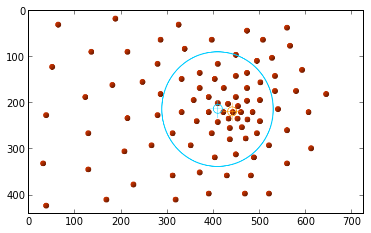
\includegraphics[width=0.7\textwidth]{meanshift_files/meanshift_fig_05.png}
\par
\end{center}
\end{codeoutput}
\end{codecell}
\begin{codecell}
\begin{codeinput}
\begin{lstlisting}
im=imread("mean_7.png"); imshow(im)

\end{lstlisting}
\end{codeinput}
\begin{codeoutput}
\begin{verbatim}
<matplotlib.image.AxesImage at 0xa2a132c>
\end{verbatim}
\begin{center}
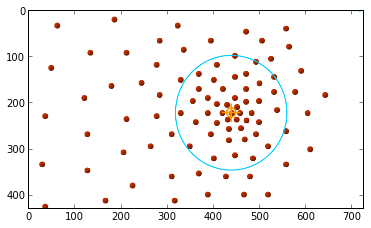
\includegraphics[width=0.7\textwidth]{meanshift_files/meanshift_fig_06.png}
\par
\end{center}
\end{codeoutput}
\end{codecell}
Fakat metodu anlatan kaynaklarda pek bahsedilmeyen bir konu var, o da
pencere icindeki diger noktalarin kume aidiyeti ve pencere ilerlerken o
pencerenin altinda olan ve olmus tum noktalarin ``bakilmis'' yani
``islenmis'' olarak addedilmesi ve bir daha ele alinmamasi. Mesela
alttaki resimde sol ust kisimdaki herhangi bir noktadan baslamissak, o
bolgedeki diger noktalar da herhalde benzer pencerelerin altina
dusecekler, ve yavas yavas, yeni ortalamalar sayesinde o pencereyi asagi
dogru itecekler, ve soldaki yogunluk merkezini bulacagiz. Ayni sey sag
tarafa da olacak. O sebeple pencere altina dusen nokta artik ayri bir
sekilde baslangic olarak islenmiyor.

Bir diger konu: ya yogunluk merkezine cok yakin bir noktadan /
noktalardan baslamissak?

O zaman ilerleme o baslangic noktasi icin aninda bitecek, cunku hemen
yogunluk merkezine gelmis olacagiz. Diger yonlerden gelen pencereler de
ayni yere gelecekler tabii, o zaman ayni / yakin yogunluk merkezlerini
ayni kume olarak kabul etmemiz gerekir. Bu ``ayni kume irdelemesi''
sayisal hesaplama acisindan ufak farklar gosterebilir tabii, ve bu ufak
farki gozonune alarak ``kume birlestirme'' mantigini da eklemek
gerekiyor.

Ortalama Kaydirma sisteminde pencere buyuklugu kullanici tarafindan
tanimlanir. Fakat bu secimin cok ``hassas'' bir ayar olmadigini gorduk
(ki bu iyi bir sey), yani pencere buyuklugunde yapilan ufak degisimlerin
bulunan kume sayisi, ve kalitesinde buyuk degisimler yaratmiyor.

\begin{codecell}
\begin{codeinput}
\begin{lstlisting}
im=imread("start.png"); imshow(im)

\end{lstlisting}
\end{codeinput}
\begin{codeoutput}
\begin{verbatim}
<matplotlib.image.AxesImage at 0x9af0f2c>
\end{verbatim}
\begin{center}
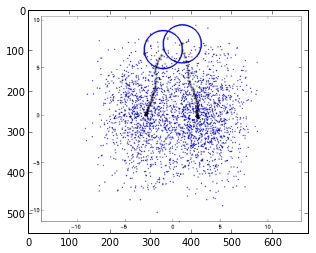
\includegraphics[width=0.7\textwidth]{meanshift_files/meanshift_fig_07.png}
\par
\end{center}
\end{codeoutput}
\end{codecell}
Altta ornek veri ve kodu bulabilirsiniz. Metot kume sayisi 17'yi
otomatik olarak buluyor.

\begin{codecell}
\begin{codeinput}
\begin{lstlisting}
from pandas import *
data = read_csv("synthetic.txt",header=None,sep="   ")
print data.shape
data = np.array(data)
\end{lstlisting}
\end{codeinput}
\begin{codeoutput}
\begin{verbatim}
(3000, 2)
\end{verbatim}
\end{codeoutput}
\end{codecell}
\begin{codecell}
\begin{codeinput}
\begin{lstlisting}
scatter(data[:,0],data[:,1])
\end{lstlisting}
\end{codeinput}
\begin{codeoutput}
\begin{verbatim}
<matplotlib.collections.PathCollection at 0x9fb632c>
\end{verbatim}
\begin{center}
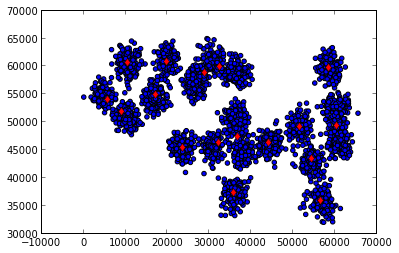
\includegraphics[width=0.7\textwidth]{meanshift_files/meanshift_fig_08.png}
\par
\end{center}
\end{codeoutput}
\end{codecell}
\begin{codecell}
\begin{codeinput}
\begin{lstlisting}
from numpy import *
from numpy import linalg as la

def mean_shift(dataPts, bandWidth):
    dataPts = asarray( dataPts )
    bandWidth = float( bandWidth )
    plotFlag = False    
    
    numDim, numPts = dataPts.shape
    numClust        = 0
    bandSq          = bandWidth**2
    initPtInds      = arange( numPts )
    #biggest size in each dimension 
    maxPos          = dataPts.max(0)
    #smallest size in each dimension                       
    minPos          = dataPts.min(0)
    #bounding box size
    boundBox        = maxPos-minPos
    #indicator of size of data space        
    sizeSpace       = la.norm(boundBox)
    #when mean has converged
    stopThresh      = 1e-3*bandWidth
    #center of clust
    clustCent       = []
    #track if a points been seen already
    beenVisitedFlag = zeros( numPts, dtype = uint8 )
    #number of points to possibly use as initilization points
    numInitPts      = numPts
    #used to resolve conflicts on cluster membership
    clusterVotes    = []
    
    while numInitPts:
        
        rand = random.rand()
        #pick a random seed point
        tempInd         = int(floor( (numInitPts-1e-6)*rand ))
        #use this point as start of mean
        stInd           = initPtInds[ tempInd ]               
        # intilize mean to this points location
        myMean          = dataPts[ :, stInd ]                 
        # points that will get added to this cluster                 
        myMembers       = []                                   
        #used to resolve conflicts on cluster membership
        thisClusterVotes    = zeros( numPts, dtype = uint16 )  
        
        while True:   
            #dist squared from mean to all points still active            
            sqDistToAll = (( myMean[:,newaxis] - dataPts )**2).sum(0)
            #points within bandWidth
            inInds      = where(sqDistToAll < bandSq)
            #add a vote for all the in points belonging to this cluster
            thisClusterVotes[ inInds ] = thisClusterVotes[ inInds ]+1 
            
            #save the old mean                        
            myOldMean   = myMean
            #compute the new mean
            myMean      = mean( dataPts[ :, inInds[0] ], 1 )
            #add any point within bandWidth to the cluster
            myMembers.extend( inInds[0] )                   
            #mark that these points have been visited
            beenVisitedFlag[myMembers] = 1                  
                        
            if la.norm(myMean-myOldMean) < stopThresh:                
                #check for merge posibilities
                mergeWith = None
                for cN in xrange( numClust ):
                    #distance from possible new clust max to old clust max
                    distToOther = la.norm( myMean - clustCent[ cN ] )    
                    #if its within bandwidth/2 merge new and old
                    if distToOther < bandWidth/2:                    
                        mergeWith = cN
                        break

                # something to merge                                
                if mergeWith is not None:
                    #record the max as the mean of the two merged (I know biased twoards new ones)
                    clustCent[ mergeWith ] = 0.5*( myMean + clustCent[ mergeWith ] )
                    #add these votes to the merged cluster
                    clusterVotes[ mergeWith ]    += thisClusterVotes   
                else:
                    #increment clusters
                    numClust                    = numClust+1
                    #record the mean  
                    clustCent.append( myMean )
                    clusterVotes.append( thisClusterVotes )
    
                break
        
        initPtInds      = where(beenVisitedFlag == 0)[0]
        numInitPts      = len(initPtInds)              
    
    data2cluster = asarray( clusterVotes ).argmax(0)                

    return clustCent, data2cluster
\end{lstlisting}
\end{codeinput}
\end{codecell}
\begin{codecell}
\begin{codeinput}
\begin{lstlisting}
dataPts = asarray([[1,1],[2,2],[3,3],[9,9],[9,9],[9,9],[10,10]]).T
print dataPts
print dataPts.shape
bandwidth = 2
print 'data points:', dataPts
print 'bandwidth:', bandwidth
clustCent, data2cluster = mean_shift(dataPts, 2)
print 'cluster centers:', sorted( asarray( clustCent ).squeeze().tolist() )
print 'data2cluster:', data2cluster
print len( clustCent )
print sorted( asarray( clustCent ).squeeze().tolist() )
\end{lstlisting}
\end{codeinput}
\begin{codeoutput}
\begin{verbatim}
[[ 1  2  3  9  9  9 10]
 [ 1  2  3  9  9  9 10]]
(2, 7)
data points: [[ 1  2  3  9  9  9 10]
 [ 1  2  3  9  9  9 10]]
bandwidth: 2
cluster centers: [[2.0, 2.0], [9.25, 9.25]]
data2cluster: [1 1 1 0 0 0 0]
2
[[2.0, 2.0], [9.25, 9.25]]
\end{verbatim}
\end{codeoutput}
\end{codecell}
\begin{codecell}
\begin{codeinput}
\begin{lstlisting}
print asarray(data.T)[:30]
clustCent, data2cluster = mean_shift(asarray(data.T), 5000)
\end{lstlisting}
\end{codeinput}
\begin{codeoutput}
\begin{verbatim}
[[54620 52694 53253 ...,  8828  8879 10002]
 [43523 42750 43024 ..., 59102 59244 61399]]
\end{verbatim}
\end{codeoutput}
\end{codecell}
\begin{codecell}
\begin{codeinput}
\begin{lstlisting}
print asarray(clustCent)[:6]
print asarray(clustCent).shape

\end{lstlisting}
\end{codeinput}
\begin{codeoutput}
\begin{verbatim}
[[ 23699.95483871  45459.8       ]
 [ 51577.72222222  49152.9691358 ]
 [ 36875.68540055  47307.43779413]
 [ 10569.30463576  60602.27152318]
 [ 19721.95906433  60651.1871345 ]
 [ 32502.45283019  59820.74339623]]
(17, 2)
\end{verbatim}
\end{codeoutput}
\end{codecell}
\begin{codecell}
\begin{codeinput}
\begin{lstlisting}
scatter(data[:,0],data[:,1])
plt.hold(True)
for x in asarray(clustCent): plot(x[0],x[1],'rd')

\end{lstlisting}
\end{codeinput}
\begin{codeoutput}
\begin{center}
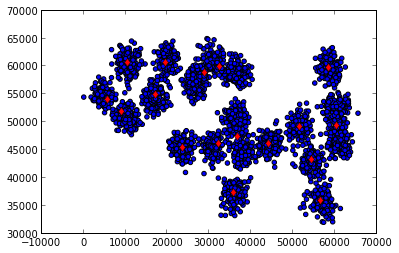
\includegraphics[width=0.7\textwidth]{meanshift_files/meanshift_fig_09.png}
\par
\end{center}
\end{codeoutput}
\end{codecell}
Teorik Konular

Bu metotu teorik bir yapiya oturtmak icin onu yazinin ilk basindaki
resimde oldugu gibi gormek gerekiyor, yani mesela o ilk resmin sagindaki
2 boyuttaki veri dagilimi (ki ayriksal, sayisal), 3 boyuttaki surekli
(continuous) bir baska dagilimin yansimasi sanki, ki o zaman 2 boyuttaki
yogunluk bolgeleri surekli dagilimdaki tepe noktalarini temsil
ediyorlar, ve biz o surekli versiyondaki tepe noktalarini bulmaliyiz.
Fakat kumeleme isleminin elinde sadece 2 boyuttaki veriler var, o zaman
surekli dagilimi bir sekilde yaratmak lazim.

Bunu yapmak icin problem / veri once bir Cekirdek Yogunluk Kestirimi
(Kernel Density Estimation -KDE-) problemi gibi goruluyor, ki her nokta
uzerine bir cekirdek fonksiyonu koyularak ve onlarin toplamim alinarak
sayisal dagilim puruzsuz bir hale getiriliyor. Ortalama Kaydirma icin
gerekli kayma ``yonu'' ise iste bu yeni surekli fonksiyonun gradyanidir
deniyor, ve gradyan yerel tepe noktasini gosterdigi icin o yone yapilan
hareket bizi yavas yavas tepeye goturecektir. Bu hareketin yerel
tepeleri bulacagi, ve tum yontemin nihai olarak sonuca yaklasacagi
(convergence) matematiksel olarak ispat edilebilir.

Tum dagilim fonksiyonunun icbukey olup olmadigi onemli degil (ki mesela
lojistik regresyonda bu onemliydi), cunku nihai tepe noktasini degil,
birkac yerel tepe noktasindan birini (hatta hepsini) bulmakla
ilgileniyoruz. Gradyan bizi bu noktaya tasiyacaktir.

Kaynaklar

http://www.serc.iisc.ernet.in/\ensuremath{\sim}venky/SE263/slides/Mean-Shift-Theory.pdf

http://saravananthirumuruganathan.wordpress.com/2010/04/01/introduction-to-mean-shift-algorithm/

http://www.cse.yorku.ca/\ensuremath{\sim}kosta/CompVis\_Notes/mean\_shift.pdf

http://homepages.inf.ed.ac.uk/rbf/CVonline/LOCAL\_COPIES/TUZEL1/MeanShift.pdf

http://yotamgingold.com/code/MeanShiftCluster.py

\end{document}
